\chapter{Kompression}\label{ch:Lektion}
\section{Einführung}

\subsection{Was ist Kompression?}

Der Begriff \enquote{Kompression} stammt --- wie viele andere Begriffe --- ursprünglich aus dem Lateinischen (\textit{compressio} $=$ das Zusammendrücken, die Zusammenpressung, die Umarmung). Mit Kompression ist also häufig die \enquote{Verkleinerung}, bzw. das \enquote{Zusammendrücken} von Daten gemeint, meist aus einem der folgenden Gründen:

\begin{enumerate}
	\item \textbf{Speicherplatz optimieren}: Angesichts des stets wachsenden Speicherbedarfs von Datenzentren sowie privaten Geräten wird es immer wichtiger, Dokumente zu \enquote{komprimieren}, d.h., deren Grösse zu verringern, falls möglich (siehe \cref{fig:compression-ex}).
	      \begin{figure}[H]
		      \centering
		      
\includegraphics[width=.6\textwidth]{Grundlagen_Info/04_Kompression/Figures/compression3}
		      \caption{Beispiel einer Datei sowie deren Dateigrösse,  unkomprimiert (original) und komprimiert}
		      \label{fig:compression-ex}
	      \end{figure}
	      \begin{figure}[H]
		      \centering
		      \raisebox{-0.5\height}{
\includegraphics[width=.2\textwidth]{Grundlagen_Info/04_Kompression/Figures/compression1}}
		      \raisebox{-0.5\height}{$\rightarrow$}
		      \raisebox{-0.5\height}{
\includegraphics[width=.25\textwidth]{Grundlagen_Info/04_Kompression/Figures/compression2}}
	      \end{figure}
	\item \textbf{Speicherplatz sparen}: Häufig kann mit wenig Aufwand Speicherplatz optimiert werden, womit der Platzbedarf auf Speichermedien wie Festplatten verringert werden kann. Da Festplatten --- ähnlich einem Reisekoffer --- Kosten verursachen, will man den Speicherbedarf möglichst minimal halten (siehe \cref{fig:speicherplatz-opt}).
	      \begin{figure}[H]
		      \centering
		      \raisebox{-0.5\height}{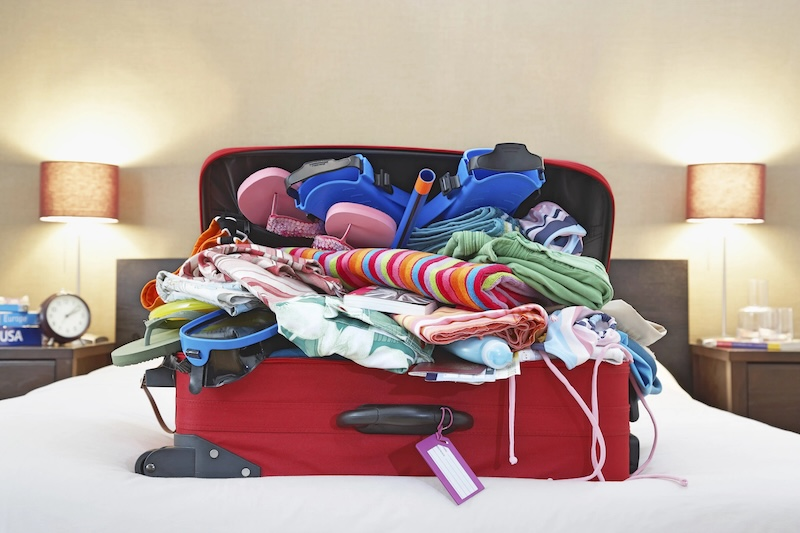
\includegraphics[width=.45\textwidth]{Grundlagen_Info/04_Kompression/Figures/messy_suitcase.jpg}}
		      \raisebox{-0.5\height}{$\rightarrow$}
		      \raisebox{-0.5\height}{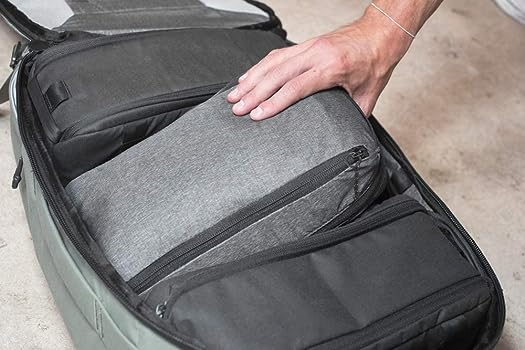
\includegraphics[width=.45\textwidth]{Grundlagen_Info/00_Programmieren/Figures/prog-packing-cubes}}
		      \caption{Speicherplatz optimieren}
		      \label{fig:speicherplatz-opt}
	      \end{figure}
	\item \textbf{Wartezeit verkürzen}: Computer und Geräte kommunizieren in Netzwerken, innerhalb welchen oftmals grosse Datenmengen übertragen werden müssen. Die Verbindungen zwischen den Geräten haben jedoch nur eine begrenzte Kapazität und werden daher häufig als \tib{Flaschenhälse} bezeichnet.
	      \begin{figure}[H]
		      \centering
		      \resizebox{!}{.5\height}{%
			      \begin{tikzpicture}
				      \path[mindmap,concept color=black,text=white]
				      node[concept] {Computer}
				      [clockwise from=0]
				      child[concept color=green!50!black] {
						      node[concept] {Computer}
							      [clockwise from=90]
						      child { node[concept] {Computer} }
						      child { node[concept] {Computer} }
						      child { node[concept] {Computer} }
						      child { node[concept] {Computer} }
					      }
				      child[concept color=blue] {
						      node[concept] {Computer}
							      [clockwise from=-30]
						      child { node[concept] {Computer} }
						      child { node[concept] {Computer} }
					      }
				      child[concept color=red] { node[concept] {Computer} }
				      child[concept color=orange] { node[concept] {Computer} };
			      \end{tikzpicture}}
		      \caption{Visualisierung von Computernetzwerken und deren \textit{Flaschenhälsen}}
	      \end{figure}
\end{enumerate}

Historischer Kontext
\begin{itemize}
	\item Leder und Stein: Teure Materialien
	\item Römische Zahlendarstellung: z.B. Zahl \textbf{999}
	      \begin{center}
		      \texttt{CCCCCCCCCXXXXXXXXXIIIIIIIII}\\
		      $\downarrow$\\
		      Erfindung der Ziffern D (500), L (50), V(5)\\
		      $\downarrow$\\
		      \texttt{DCCCCLXXXXVIIII} \\
		      $\downarrow$\\
		      Effizientere Schreibweise\\
		      $\downarrow$\\
		      IM
	      \end{center}
\end{itemize}

\section{Verlustfreie vs. verlustbehaftete Kompression}
Einige Beispiele:
\begin{table}[H]
	\centering
	\begin{tabular}{c||c|c}
		\textbf{Anwendung}  & \textbf{Verlustfrei}                        & \textbf{Verlustbehaftet}                    \\\midrule
		\textbf{Audio}      & \texttt{.flac, .wav}                        & \texttt{.mp3, .aac}                         \\\hline
		\textbf{Dateien}    & \texttt{.zip}, \texttt{.rar}                & \texttt{-}                                  \\\hline
		\textbf{Video}      & \texttt{.raw}                               & \texttt{.mp4}, \texttt{.avi}, \texttt{.mov} \\\hline
		\textbf{Fotografie} & \texttt{.raw}, \texttt{.psd}, \texttt{.png} & \texttt{.jpg}, \texttt{.webp}              \\\hline
		\textbf{Grafik}     & \texttt{.svg}, \texttt{.pdf}                & \texttt{-}
	\end{tabular}
\end{table}

\begin{figure}
	\centering
	\begin{subfigure}{.45\linewidth}
		\begin{tikzpicture}[boximg]
			\node[anchor=south west] (img) {
\includegraphics[width=\linewidth]{{Grundlagen_Info/04_Kompression/Figures/LeeLogo 300 dpi.jpg}}};
			\begin{scope}[x=(img.south east),y=(img.north west)]
				\node[draw,minimum height=.3cm,minimum width=.75cm] (B1) at (0.48,0.47) {};
			\end{scope}
		\end{tikzpicture}
		\caption{}
	\end{subfigure}\\[0.5\baselineskip]
	\begin{subfigure}{\linewidth}
		\begin{tikzpicture}[boximg]
			\node (img1) {
\includegraphics[width=0.9\linewidth]{Grundlagen_Info/04_Kompression/Figures/LeeLogo 300 dpi zoom}};
			\draw (img1.south west) rectangle (img1.north east);
		\end{tikzpicture}\hfill%
		\caption{}
	\end{subfigure}
	\begin{tikzpicture}[overlay,boximg]
		\draw (B1) -- (img1);
	\end{tikzpicture}
	\caption{\texttt{LeeLogo\textbf{.jpg} (48 KB, 300 dots per inch)}}
\end{figure}



\section{Kompressionsalgorithmen}

\begin{myexercise}
	Was könnte folgende Sequenz bedeuten?
	\begin{center}
		WENN \emoji{blush} HINTER \emoji{blush} $\triangle$, $\triangle$ EINIGE \emoji{blush} ANDEREN \emoji{blush} NACH.
	\end{center}
	\begin{myanswer}
		Viele Bedeutungen sind möglich, zum Beispiel:
		\begin{center}
			WENN GRIECHEN HINTER GRIECHEN RENNEN, RENNEN EINIGE GRIECHEN ANDEREN GRIECHEN NACH.
		\end{center}
	\end{myanswer}
\end{myexercise}

Wie können wir folgenden Text effizient kodieren?

\begin{center}
	AACABAAACBACAACADAAD
\end{center}

Da wir hier nur vier Buchstaben (A, B, C und D) haben, reichen 2 Bits für die Kodierung aus, da 2 Bits $2^2=4$ Möglichkeiten zur Kodierung bieten.

\begin{table}[H]
	\centering
	\begin{tabular}{c|c|c|c|c}
		\textbf{Buchstabe}        & \textbf{A} & \textbf{B} & \textbf{C} & \textbf{D} \\\midrule\midrule
		Häufigkeit                & 12         & 2          & 4          & 2          \\\hline
		Relative Häufigkeit       & 60\%       & 10\%       & 20\%       & 10\%       \\\hline
		\enquote{Naive} Kodierung:      & 00         & 01         & 10         & 11         \\\hline
		\enquote{Effiziente} Kodierung: & 0          & 110        & 10         & 111        \\
	\end{tabular}
\end{table}
\begin{itemize}
	\item \enquote{Naive} Codierung (40 Zeichen):\\ \texttt{0000100001000000100100100000100011000011}
	\item \enquote{Effiziente} Codierung (32 Zeichen, -20\% Ersparnis):\\ \texttt{0010110000101100100010011100111}\\

\end{itemize}

Die \enquote{effiziente} Kodierung verwendet in diesem Fall 20\% weniger Speicherplatz als die \enquote{naive} Kodierung.

Beide Codierungen sind \textbf{präfixfrei}: Kein Codewort ist Anfangsstück (Präfix) eines anderen Codeworts. Dies ist notwendig, damit es keine Verwechslungsgefahr beim Interpretieren des Codes gibt.

\begin{myexercise}
	Wir haben einen Text mit 100 Buchstaben und den Buchstaben A, B, C, D sowie E. Im Text kommt A 55-mal, D und E jeweils 20-mal, B 3-mal und C 2-mal vor. Wählen Sie eine präfixfreie Kodierung der 5 Buchstaben des Alphabets, sodass die resultierende binäre Darstellung des Textes so kurz wie möglich wird.
	\begin{enumerate}
		\item Visualisieren Sie den Prozess bei der Wahl der Kodierungen der einzelnen Buchstaben mit einem Baumdiagramm.
		\item  Wie lange ist die binäre Darstellung des Texts mit Ihrer Kodierung?
	\end{enumerate}
	\begin{myanswer}
		Eine mögliche Lösung:
		\begin{figure}[H]
			\centering
			\begin{tikzpicture}
				[-,>=stealth',
					level distance=18mm,
					level 1/.style={sibling distance=60mm},
					level 2/.style={sibling distance=30mm},
					level 3/.style={sibling distance=15mm},
					level 4/.style={sibling distance=8mm},
					leaf/.style={circle, draw},
					label/.style={red},
					edge from parent path={(\tikzparentnode.south) -- (\tikzchildnode)}]


				\usetikzlibrary{shapes}
				\tikzstyle{n} = [text width=1cm,align=center]
				\tikzstyle{r} = [text=red]

				\node[n]{\textcolor{RoyalBlue}{A,B,C,D,E}\\ 100\%}[edge from parent]
				child {node[n] {\textcolor{RoyalBlue}{A}\\ 55\%\\\textcolor{red}{0}}
						edge from parent node[left,r]{0};
					}
				child {node[n]{\textcolor{RoyalBlue}{B,C,D,E}\\ 45\%}
						child {node[n] {\textcolor{RoyalBlue}{D}\\ 20\%\\\textcolor{red}{10}}
								edge from parent[] node[left,r]{0};
							}
						child {node[n] {\textcolor{RoyalBlue}{B,C,E}\\ 25\%}
								child {node[n] {\textcolor{RoyalBlue}{E}\\20\%\\\textcolor{red}{110}}
										edge from parent[] node[left,r]{0};
									}
								child {node[n] {\textcolor{RoyalBlue}{B,C}\\ 5\%}
										child {node[n] {\textcolor{RoyalBlue}{B}\\3\%\\\textcolor{red}{1110}}
												edge from parent[] node[left,r]{0};
											}
										child {node[n] {\textcolor{RoyalBlue}{C}\\ 2\%\\\textcolor{red}{1111}}
												edge from parent[] node[r,right]{1};
											}
										edge from parent[] node[r,right]{1};
									}
								edge from parent[] node[r,right]{1};
							}
						edge from parent node[r,right]{1};
					};
			\end{tikzpicture}
		\end{figure}
		Die Länge des gesamten Texts berechnet sich aus der Summe der Häufigkeiten der Buchstaben mal deren Kodierungslänge:
		\begin{table}[H]
			\centering
			\begin{tabular}{c||c|c}
				Buchstabe & Kodierung & Länge der Kodierung \\\midrule\midrule
				A         & 0         & 1                   \\\midrule
				B         & 1110      & 4                   \\\midrule
				C         & 1111      & 4                   \\\midrule
				D         & 10        & 2                   \\\midrule
				E         & 110       & 3
			\end{tabular}
		\end{table}
		\[55\times1+3\times4 + 2\times4 + 20\times2 + 20\times3 = 175\]
	\end{myanswer}
\end{myexercise}

\begin{table}[H]
	\centering
	\begin{tabular}{c|c|c|c|c}
		\textbf{Buchstabe}        & \textbf{A} & \textbf{B} & \textbf{C} & \textbf{D} \\\midrule\midrule
		Relative Häufigkeit       & 60\%       & 10\%       & 20\%       & 10\%       \\\hline
		\enquote{Effiziente} Kodierung: & 0          & 110        & 10         & 111        \\
	\end{tabular}
\end{table}
\begin{figure}[H]
	\centering
	\begin{tikzpicture}
		[-,>=stealth',level distance=15mm,
			level 1/.style={sibling distance=60mm},
			level 2/.style={sibling distance=30mm},
			level 3/.style={sibling distance=15mm},
			level 4/.style={sibling distance=15mm}, leaf/.style={circle, draw}, label/.style={red},edge from parent path={(\tikzparentnode.south) -- (\tikzchildnode)}]


		\usetikzlibrary{shapes}
		\tikzstyle{c} = [draw, shape=circle]
		\tikzstyle{n} = [text width=1cm,align=center]
		\tikzstyle{r} = [text=red]

		\node[]{}[edge from parent]
		child {node[n] {A\\ \textcolor{red}{0}}
				edge from parent coordinate (ea);
			}
		child {node[]{}
				child {node[text width=1cm,align=center]{C\\ \textcolor{red}{10}}
						edge from parent coordinate (e25);
					}
				child {node[]{}
						child{node[n]{B\\ \textcolor{red}{110}}
								edge from parent coordinate (e14);
							}
						child{node[n]{D \\ \textcolor{red}{111}}
								edge from parent coordinate (e16);
							}
						edge from parent coordinate (e30);
					}
				edge from parent coordinate (e55);
			};
		% code labels
		\node[r] at([yshift=2mm]ea)  {0};
		\node[r] at([yshift=2mm]e55) {1};
		\node[r] at([xshift=-2mm,yshift=2mm]e25) {0};
		\node[r] at([xshift=2mm,yshift=2mm]e30) {1};
		\node[r] at([xshift=-2mm,yshift=1mm]e14) {0};
		\node[r] at([xshift=2mm,yshift=1mm]e16) {1};
	\end{tikzpicture}
\end{figure}

\subsection{Top-Down-Ansatz: Maximale Balance}
\textbf{Idee}: Summe der Buchstabenhäufigkeiten im linken und rechten Teilbaum ausbalancieren

\begin{table}[H]
	\centering
	\begin{tabular}{c|c|c|c|c|c|c}
		\textbf{Buchstabe}  & \textbf{A} & \textbf{B} & \textbf{C} & \textbf{D} & \textbf{E} & \textbf{F} \\\midrule\midrule
		Relative Häufigkeit & 25\%       & 25\%       & 13\%       & 13\%       & 12\%       & 12\%
	\end{tabular}
	\caption{Beispiel-Häufigkeiten von Buchstaben}
	\label{table:ex-topdown}
\end{table}

\begin{figure}[H]
	\centering
	\begin{subfigure}{.49\textwidth}
		\centering
		\begin{tikzpicture}
			[-,>=stealth',
				level distance=18mm,
				level 1/.style={sibling distance=30mm},
				level 2/.style={sibling distance=30mm},
				level 3/.style={sibling distance=15mm},
				level 4/.style={sibling distance=8mm},
				leaf/.style={circle, draw},
				label/.style={red},
				edge from parent path={(\tikzparentnode.south) -- (\tikzchildnode)},
				background rectangle/.style={fill=black!3,rounded corners},
				show background rectangle]


			\usetikzlibrary{shapes}
			\tikzstyle{n} = [text width=1cm,align=center]
			\tikzstyle{r} = [text=red]

			\node[n]{\textcolor{RoyalBlue}{A,B,C,D,E,F}\\ 100\%}[edge from parent]
			child {node[n] {\textcolor{RoyalBlue}{A,B}\\ 50\%}
					edge from parent node[left,r]{0};
				}
			child {node[n]{\textcolor{RoyalBlue}{C,D,E,F}\\ 50\%}
					edge from parent node[r,right]{1};
				};
		\end{tikzpicture}
		\caption{Schritt 1}
	\end{subfigure}
	\hfill
	\begin{subfigure}{.49\textwidth}
		\centering
		\begin{tikzpicture}
			[-,>=stealth',
				level distance=18mm,
				level 1/.style={sibling distance=30mm},
				level 2/.style={sibling distance=30mm},
				level 3/.style={sibling distance=15mm},
				level 4/.style={sibling distance=8mm},
				leaf/.style={circle, draw},
				label/.style={red},
				edge from parent path={(\tikzparentnode.south) -- (\tikzchildnode)},background rectangle/.style={fill=black!3,rounded corners}, show background rectangle]


			\usetikzlibrary{shapes}
			\tikzstyle{n} = [text width=1cm,align=center]
			\tikzstyle{r} = [text=red]

			\node[n]{\textcolor{RoyalBlue}{A,B,C,D,E,F}\\ 100\%}[edge from parent]
			child {node[n] {\textcolor{RoyalBlue}{A,B}\\ 50\%}
					child {node[n] {\textcolor{RoyalBlue}{A}\\ 25\%\\\textcolor{red}{00}}
							edge from parent[] node[left,r]{0};
						}
					child {node[n] {\textcolor{RoyalBlue}{B}\\ 25\%\\\textcolor{red}{01}}
							edge from parent[] node[r,right]{1};
						}
					edge from parent node[left,r]{0};
				}
			child {node[n]{\textcolor{RoyalBlue}{C,D,E,F}\\ 50\%}
					edge from parent node[r,right]{1};
				};
		\end{tikzpicture}
		\caption{Schritt 2}
	\end{subfigure}
	\begin{subfigure}{\textwidth}
		\centering
		\begin{tikzpicture}
			[-,>=stealth',
				level distance=18mm,
				level 1/.style={sibling distance=60mm},
				level 2/.style={sibling distance=30mm},
				level 3/.style={sibling distance=15mm},
				level 4/.style={sibling distance=8mm},
				leaf/.style={circle, draw},
				label/.style={red},
				edge from parent path={(\tikzparentnode.south) -- (\tikzchildnode)},background rectangle/.style={fill=black!3,rounded corners}, show background rectangle]


			\usetikzlibrary{shapes}
			\tikzstyle{n} = [text width=1cm,align=center]
			\tikzstyle{r} = [text=red]

			\node[n]{\textcolor{RoyalBlue}{A,B,C,D,E,F}\\ 100\%}[edge from parent]
			child {node[n] {\textcolor{RoyalBlue}{A,B}\\ 50\%}
					child {node[n] {\textcolor{RoyalBlue}{A}\\ 25\%\\\textcolor{red}{00}}
							edge from parent[] node[left,r]{0};
						}
					child {node[n] {\textcolor{RoyalBlue}{B}\\ 25\%\\\textcolor{red}{01}}
							edge from parent[] node[r,right]{1};
						}
					edge from parent node[left,r]{0};
				}
			child {node[n]{\textcolor{RoyalBlue}{C,D,E,F}\\ 50\%}
					child {node[n] {\textcolor{RoyalBlue}{C,E}\\ 25\%}
							edge from parent[] node[left,r]{0};
						}
					child {node[n] {\textcolor{RoyalBlue}{D,F}\\ 25\%}
							edge from parent[] node[r,right]{1};
						}
					edge from parent node[r,right]{1};
				};
		\end{tikzpicture}
		\caption{Schritt 3}
	\end{subfigure}

	\begin{subfigure}{\textwidth}
		\centering
		\begin{tikzpicture}
			[-,>=stealth',
				level distance=18mm,
				level 1/.style={sibling distance=60mm},
				level 2/.style={sibling distance=30mm},
				level 3/.style={sibling distance=15mm},
				level 4/.style={sibling distance=8mm},
				leaf/.style={circle, draw},
				label/.style={red},
				edge from parent path={(\tikzparentnode.south) -- (\tikzchildnode)},background rectangle/.style={fill=black!3,rounded corners}, show background rectangle]


			\usetikzlibrary{shapes}
			\tikzstyle{n} = [text width=1cm,align=center]
			\tikzstyle{r} = [text=red]

			\node[n]{\textcolor{RoyalBlue}{A,B,C,D,E,F}\\ 100\%}[edge from parent]
			child {node[n] {\textcolor{RoyalBlue}{A,B}\\ 50\%}
					child {node[n] {\textcolor{RoyalBlue}{A}\\ 25\%\\\textcolor{red}{00}}
							edge from parent[] node[left,r]{0};
						}
					child {node[n] {\textcolor{RoyalBlue}{B}\\ 25\%\\\textcolor{red}{01}}
							edge from parent[] node[r,right]{1};
						}
					edge from parent node[left,r]{0};
				}
			child {node[n]{\textcolor{RoyalBlue}{C,D,E,F}\\ 50\%}
					child {node[n] {\textcolor{RoyalBlue}{C,E}\\ 25\%}
							child {node[n] {\textcolor{RoyalBlue}{C}\\ 13\%\\\textcolor{red}{100}}
									edge from parent[] node[left,r]{0};
								}
							child {node[n] {\textcolor{RoyalBlue}{E}\\ 12\%\\\textcolor{red}{101}}
									edge from parent[] node[r,right]{1};
								}
							edge from parent[] node[left,r]{0};
						}
					child {node[n] {\textcolor{RoyalBlue}{D,F}\\ 25\%}
							child {node[n] {\textcolor{RoyalBlue}{D}\\ 13\%\\\textcolor{red}{110}}
									edge from parent[] node[left,r]{0};
								}
							child {node[n] {\textcolor{RoyalBlue}{F}\\ 12\%\\\textcolor{red}{111}}
									edge from parent[] node[r,right]{1};
								}
							edge from parent[] node[r,right]{1};
						}
					edge from parent node[r,right]{1};
				};
		\end{tikzpicture}
		\caption{Schritt 4 (Kodierung)}
	\end{subfigure}
	\caption{Schritt-für-Schritt-Erstellung des Baumdiagramms für \cref{table:ex-topdown} mit dem \tib{Top-Down}-Ansatz.}
\end{figure}

\begin{myexercise}
	Nutzen Sie die Strategie der maximalen Balance, um die präfixfreien Kodierungen für Texte
	mit folgenden Buchstabenhäufigkeiten zu entwerfen.
	\begin{enumerate}
		\item A - 57\%, B - 23\%, C - 12\%, D - 8\%
		\item A - 25\%, B - 20 \%, D - 14 \%, E - 11 \%, F - 10 \%, G - 10 \%, H - 5\%, I - 5\%
		\item A - 33 \%, B - 30 \%, C - 17 \%, D - 14 \%, E - 6\%
	\end{enumerate}

	\begin{myanswer}
		\begin{figure}[H]
			\centering
			\begin{tikzpicture}
				[-,>=stealth',
					level distance=18mm,
					level 1/.style={sibling distance=60mm},
					level 2/.style={sibling distance=30mm},
					level 3/.style={sibling distance=15mm},
					level 4/.style={sibling distance=8mm},
					leaf/.style={circle, draw},
					label/.style={red},
					edge from parent path={(\tikzparentnode.south) -- (\tikzchildnode)},background rectangle/.style={fill=black!3,rounded corners}, show background rectangle]


				\usetikzlibrary{shapes}
				\tikzstyle{n} = [text width=1cm,align=center]
				\tikzstyle{r} = [text=red]

				\node[n]{\textcolor{RoyalBlue}{A,B,C,D}\\ 100\%}[edge from parent]
				child {node[n] {\textcolor{RoyalBlue}{A}\\ 57\%\\\textcolor{red}{0}}
						edge from parent node[left,r]{0};
					}
				child {node[n]{\textcolor{RoyalBlue}{B,C,D}\\ 43\%}
						child {node[n] {\textcolor{RoyalBlue}{C,D}\\ 20\%}
								child {node[n] {\textcolor{RoyalBlue}{C}\\ 12\%\\\textcolor{red}{100}}
										edge from parent[] node[left,r]{0};
									}
								child {node[n] {\textcolor{RoyalBlue}{D}\\ 8\%\\\textcolor{red}{101}}
										edge from parent[] node[r,right]{1};
									}
								edge from parent[] node[left,r]{0};
							}
						child {node[n] {\textcolor{RoyalBlue}{B}\\ 23\%\\\textcolor{red}{11}}
								edge from parent[] node[r,right]{1};
							}
						edge from parent node[r,right]{1};
					};
			\end{tikzpicture}
			\caption{Lösungsvorschlag für Teilaufgabe 1}
		\end{figure}
	\end{myanswer}

	\begin{myanswer}
		Für Teilaufgabe 2 gibt es mehrere Lösungsmöglichkeiten, z.B.:
		\begin{figure}[H]
			\centering
			\begin{tikzpicture}
				[-,>=stealth',
					level distance=18mm,
					level 1/.style={sibling distance=60mm},
					level 2/.style={sibling distance=30mm},
					level 3/.style={sibling distance=15mm},
					level 4/.style={sibling distance=8mm},
					leaf/.style={circle, draw},
					label/.style={red},
					edge from parent path={(\tikzparentnode.south) -- (\tikzchildnode)},background rectangle/.style={fill=black!3,rounded corners}, show background rectangle]


				\usetikzlibrary{shapes}
				\tikzstyle{n} = [text width=1cm,align=center]
				\tikzstyle{r} = [text=red]

				\node[n]{\textcolor{RoyalBlue}{A,B,D,E,F,G,H,I}\\ 100\%}[edge from parent]
				child {node[n] {\textcolor{RoyalBlue}{A,D,E}\\ 50\%}
						child {node[n] {\textcolor{RoyalBlue}{A}\\ 25\%\\\textcolor{red}{00}}
								edge from parent[] node[left,r]{0};
							}
						child {node[n] {\textcolor{RoyalBlue}{D,E}\\ 25\%}
								child {node[n] {\textcolor{RoyalBlue}{D}\\ 14\%\\\textcolor{red}{010}}
										edge from parent[] node[left,r]{0};
									}
								child {node[n] {\textcolor{RoyalBlue}{E}\\ 11\%\\\textcolor{red}{011}}
										edge from parent[] node[r,right]{1};
									}
								edge from parent[] node[r,right]{1};
							}
						edge from parent node[left,r]{0};
					}
				child {node[n]{\textcolor{RoyalBlue}{B,F,G,H,I}\\ 50\%}
						child {node[n] {\textcolor{RoyalBlue}{B,H}\\ 25\%}
								child {node[n] {\textcolor{RoyalBlue}{B}\\ 20\%\\\textcolor{red}{100}}
										edge from parent[] node[left,r]{0};
									}
								child {node[n] {\textcolor{RoyalBlue}{H}\\ 5\%\\\textcolor{red}{101}}
										edge from parent[] node[r,right]{1};
									}
								edge from parent[] node[left,r]{0};
							}
						child {node[n] {\textcolor{RoyalBlue}{F,G,I}\\ 25\%}
								child {node[n] {\textcolor{RoyalBlue}{F,I}\\ 15\%}
										child {node[n] {\textcolor{RoyalBlue}{F}\\ 10\%\\\textcolor{red}{1100}}
												edge from parent[] node[left,r]{0};
											}
										child {node[n] {\textcolor{RoyalBlue}{I}\\ 5\%\\\textcolor{red}{1101}}
												edge from parent[] node[r,right]{1};
											}
										edge from parent[] node[left,r]{0};
									}
								child {node[n] {\textcolor{RoyalBlue}{G}\\ 10\%\\\textcolor{red}{111}}
										edge from parent[] node[r,right]{1};
									}
								edge from parent[] node[r,right]{1};
							}
						edge from parent node[r,right]{1};
					};
			\end{tikzpicture}
			\caption{Lösungsvorschlag für Teilaufgabe 2}
		\end{figure}
	\end{myanswer}

	\begin{myanswer}
		\begin{figure}[H]
			\centering
			\begin{tikzpicture}
				[-,>=stealth',
					level distance=18mm,
					level 1/.style={sibling distance=60mm},
					level 2/.style={sibling distance=30mm},
					level 3/.style={sibling distance=15mm},
					level 4/.style={sibling distance=8mm},
					leaf/.style={circle, draw},
					label/.style={red},
					edge from parent path={(\tikzparentnode.south) -- (\tikzchildnode)},background rectangle/.style={fill=black!3,rounded corners}, show background rectangle]


				\usetikzlibrary{shapes}
				\tikzstyle{n} = [text width=1cm,align=center]
				\tikzstyle{r} = [text=red]

				\node[n]{\textcolor{RoyalBlue}{A,B,C,D,E}\\ 100\%}[edge from parent]
				child {node[n] {\textcolor{RoyalBlue}{A,C}\\ 50\%\\}
						child {node[n] {\textcolor{RoyalBlue}{A}\\ 33\%\\\textcolor{red}{00}}
								edge from parent[] node[left,r]{0};
							}
						child {node[n] {\textcolor{RoyalBlue}{C}\\ 17\%\\\textcolor{red}{01}}
								edge from parent[] node[r,right]{1};
							}
						edge from parent node[left,r]{0};
					}
				child {node[n]{\textcolor{RoyalBlue}{B,D,E}\\ 50\%}
						child {node[n] {\textcolor{RoyalBlue}{D,E}\\ 20\%}
								child {node[n] {\textcolor{RoyalBlue}{D}\\ 14\%\\\textcolor{red}{100}}
										edge from parent[] node[left,r]{0};
									}
								child {node[n] {\textcolor{RoyalBlue}{E}\\ 6\%\\\textcolor{red}{101}}
										edge from parent[] node[r,right]{1};
									}
								edge from parent[] node[left,r]{0};
							}
						child {node[n] {\textcolor{RoyalBlue}{B}\\ 30\%\\\textcolor{red}{11}}
								edge from parent[] node[r,right]{1};
							}
						edge from parent node[r,right]{1};
					};
			\end{tikzpicture}
			\caption{Lösungsvorschlag für Teilaufgabe 3}
		\end{figure}
	\end{myanswer}

\end{myexercise}

\begin{mychallenge}
	Schlagen Sie eine Häufigkeitsverteilung für Buchstaben so vor, dass die Strategie der maximalen Balance eindeutig ein Baumdiagramm bestimmt, in dem ein 10-mal häufigerer Buchstabe eine längere Kodierung hat als ein 10-mal seltener vorkommender Buchstabe.
\end{mychallenge}

\begin{myexercise}
	\textbf{Problem}: Was passiert bei folgender Verteilung?
	\begin{table}[H]
		\centering
		\begin{tabular}{c|c|c|c|c|c|c}
			\textbf{Buchstabe}  & \textbf{A} & \textbf{B} & \textbf{C} & \textbf{D} & \textbf{E} & \textbf{F} \\\midrule\midrule
			Relative Häufigkeit & 55\%       & 1\%        & 25\%       & 8\%        & 9\%        & 8\%
		\end{tabular}
	\end{table}


	\begin{myanswer}
		\begin{figure}[H]
			\centering
			\begin{tikzpicture}
				[-,>=stealth',
					level distance=15mm,
					level 1/.style={sibling distance=60mm},
					level 2/.style={sibling distance=30mm},
					level 3/.style={sibling distance=15mm},
					level 4/.style={sibling distance=15mm},
					level 5/.style={sibling distance=15mm},
					leaf/.style={circle, draw},
					label/.style={red},
					edge from parent path={(\tikzparentnode.south) -- (\tikzchildnode)},background rectangle/.style={fill=black!3,rounded corners}, show background rectangle]


				\usetikzlibrary{shapes}
				\tikzstyle{n} = [text width=1cm,align=center]
				\tikzstyle{r} = [text=red]

				\node[n]{\textcolor{RoyalBlue}{A,B,C,D,E,F}\\ 100\%}[edge from parent]
				child {node[n] {\textcolor{RoyalBlue}{A,B}\\ 50\%}
						child {node[n] {\textcolor{RoyalBlue}{A}\\55\%\\\textcolor{red}{00}}
								edge from parent[] node[left,r]{0};
							}
						child {node[n, draw] {\textcolor{RoyalBlue}{B}\\ 1\%\\\textcolor{red}{01}}
								edge from parent[] node[r,right]{1};
							}
						edge from parent node[left,r]{0};
					}
				child {node[n]{\textcolor{RoyalBlue}{C,D,E,F}\\ 50\%}
						child {node[n] {\textcolor{RoyalBlue}{C}\\ 25\%\\\textcolor{red}{10}}
								edge from parent[] node[left,r]{0};
							}
						child {node[n] {\textcolor{RoyalBlue}{D,E,F}\\ 25\%}
								child {node[n] {\textcolor{RoyalBlue}{D,E}\\ 17\%\\}
										child {node[n, draw] {\textcolor{RoyalBlue}{D}\\ 8\%\\\textcolor{red}{1100}}
												edge from parent[] node[left,r]{0};
											}
										child {node[n, draw] {\textcolor{RoyalBlue}{E}\\ 9\%\\\textcolor{red}{1101}}
												edge from parent[] node[right,r]{1};
											}
										edge from parent[] node[left,r]{0};
									}
								child {node[n, draw] {\textcolor{RoyalBlue}{F}\\ 8\%\\\textcolor{red}{111}}
										edge from parent[] node[r,right]{1};
									}
								edge from parent[] node[r,right]{1};
							}
						edge from parent node[r,right]{1};
					};
			\end{tikzpicture}
		\end{figure}
		Wie wir sehen, wird der resultierende Baum nicht ausgeglichen: während der Buchstabe \enquote{F} (8\% Häufigkeit im Originaltext) beispielsweise mit \enquote{111} kodiert wird, wird der Buchstabe \enquote{B} (1 \% Häufigkeit im Originaltext) mit \enquote{01} kodiert, also mit einer kürzeren Bitfolge. Wie wir allerdings gesehen haben, sollten Buchstaben mit höherer Häufigkeit kürzer kodiert werden, da wir sie ja häufiger kodieren müssen und mit einer kürzeren Kodierungslänge somit insgesamt mehr Speicherplatz sparen.
	\end{myanswer}

\end{myexercise}
\subsection{Bottom-Up-Ansatz: Huffman-Kodierung}

Idee:
\begin{itemize}
	\item Jeder Buchstabe wird als Graph mit einem Knoten (=Baum mit einem Blatt) betrachtet. Die Häufigkeit jedes Buchstabens wird neben dem Blatt notiert. Wir wollen nun die Buchstaben zu Teilbäumen verbinden, bis wir einen einzigen Baum haben.
	      \begin{figure}[H]
		      \centering
		      \begin{tikzpicture}[background rectangle/.style={fill=black!3,rounded corners}, show background rectangle]
			      \tikzstyle{n} = [text width=1cm,align=center, draw, shape=circle]
			      \node[circle,draw, label={[align=center]below:\textcolor{RoyalBlue}{A}\\55\%}, ](a){};
			      \node[circle,draw, label={[align=center]below:\textcolor{RoyalBlue}{B}\\ 1\%}, right of=a](b){};
			      \node[circle,draw, label={[align=center]below:\textcolor{RoyalBlue}{C}\\ 25\%}, right of=b](c){};
			      \node[circle,draw, label={[align=center]below:\textcolor{RoyalBlue}{D}\\ 8\%}, right of=c](d){};
			      \node[circle,draw, label={[align=center]below:\textcolor{RoyalBlue}{E}\\ 9\%}, right of=d](e){};
			      \node[circle,draw, label={[align=center]below:\textcolor{RoyalBlue}{F}\\ 8\%}, right of=e](f){};
		      \end{tikzpicture}
		      \caption{Beispiel-Häufigkeiten von Buchstaben}
		      \label{fig:exFreqHuffman}
	      \end{figure}
	\item In einer Schleife: Wir schauen alle isolierten Blätter und Wurzeln von Teilbäumen an. Diejenigen  Knoten, die die kleinste (gemeinsame) Prozentzahl enthalten werden miteinander verbunden. Die neue Wurzel wird markiert mit dem Prozentsatz beider Knoten.
	      \begin{figure}[H]
		      \centering
		      \begin{tikzpicture}[-,>=stealth',
				      level distance=12mm,
				      level 1/.style={sibling distance=15mm},
				      level 2/.style={sibling distance=30mm},
				      level 3/.style={sibling distance=15mm},
				      level 4/.style={sibling distance=15mm},
				      level 5/.style={sibling distance=15mm},
				      leaf/.style={circle, draw},
				      edge from parent path={(\tikzparentnode.south) -- (\tikzchildnode)},background rectangle/.style={fill=black!3,rounded corners}, show background rectangle]


			      \usetikzlibrary{shapes}
			      \tikzstyle{n} = [text width=1cm,align=center]
			      \tikzstyle{r} = [text=red]

			      \node[n]{\textcolor{RoyalBlue}{B,D}\\ 9\%}[edge from parent]
			      child {node[n] {\textcolor{RoyalBlue}{B}\\ 1\%}
					      edge from parent node[left,r]{};
				      }
			      child {node[n]{\textcolor{RoyalBlue}{D}\\ 8\%}
					      edge from parent node[r,right]{};
				      };
		      \end{tikzpicture}
		      \caption{Erster Schritt im Huffman-Kodierungs-Algorithmus}
	      \end{figure}
	\item Falls mehrere Möglichkeiten mit gleicher relativer Häufigkeit existieren, nehmen wir den Teilbaum mit der geringsten Tiefe.
\end{itemize}
\textbf{Welche Knoten werden als nächstes miteinander verbunden?}

\begin{figure}[H]
	\centering
	\begin{subfigure}{.45\textwidth}
		\begin{tikzpicture}[-,>=stealth',
				level distance=12mm,
				level 1/.style={sibling distance=15mm},
				level 2/.style={sibling distance=30mm},
				level 3/.style={sibling distance=15mm},
				level 4/.style={sibling distance=15mm},
				level 5/.style={sibling distance=15mm},
				leaf/.style={circle, draw},
				edge from parent path={(\tikzparentnode.south) -- (\tikzchildnode)},background rectangle/.style={fill=black!3,rounded corners}, show background rectangle]


			\usetikzlibrary{shapes}
			\tikzstyle{n} = [text width=1cm,align=center]
			\tikzstyle{r} = [text=red]

			\node[n]{\textcolor{RoyalBlue}{B,D}\\ 9\%}[edge from parent]
			child {node[n] (b){\textcolor{RoyalBlue}{B}\\ 1\%}
					edge from parent node[left,r]{};
				}
			child {node[n]{\textcolor{RoyalBlue}{D}\\ 8\%}
					edge from parent node[r,right]{};
				};
			\node[n, left of=b](e){\textcolor{RoyalBlue}{E}\\ 9\%};
			\node[n, left of=e](f){\textcolor{RoyalBlue}{F}\\8\%};
			\node[n, left of=f](c){\textcolor{RoyalBlue}{C}\\ 25\%};
			\node[n, left of=c](a){\textcolor{RoyalBlue}{A}\\55\%};
		\end{tikzpicture}
		\caption{Schritt 1}
	\end{subfigure}\hfill
	\begin{subfigure}{.45\textwidth}
		\begin{tikzpicture}[-,>=stealth',
				level distance=15mm,
				level 1/.style={sibling distance=15mm},
				level 2/.style={sibling distance=30mm},
				level 3/.style={sibling distance=15mm},
				level 4/.style={sibling distance=15mm},
				level 5/.style={sibling distance=15mm},
				leaf/.style={circle, draw},
				edge from parent path={(\tikzparentnode.south) -- (\tikzchildnode)},background rectangle/.style={fill=black!3,rounded corners}, show background rectangle]


			\usetikzlibrary{shapes}
			\tikzstyle{n} = [text width=1cm,align=center]
			\tikzstyle{r} = [text=red]

			\node(bd)[n]{\textcolor{RoyalBlue}{B,D}\\ 9\%}[edge from parent]
			child {node(b)[n] {\textcolor{RoyalBlue}{B}\\ 1\%}
					edge from parent node[left,r]{} ;
				}
			child {node[n]{\textcolor{RoyalBlue}{D}\\ 8\%}
					edge from parent node[r,right]{};
				};
			\node(ef)[n, left of=bd,xshift=-15mm]{\textcolor{RoyalBlue}{E,F}\\ 17\%}[edge from parent]
			child {node(f)[n] {\textcolor{RoyalBlue}{F}\\ 8\%}
					edge from parent node[left,r]{} ;
				}
			child {node[n]{\textcolor{RoyalBlue}{E}\\ 9\%}
					edge from parent node[r,right]{};
				};
			\node[n, left of=f](c){\textcolor{RoyalBlue}{C}\\ 25\%};
			\node[n, left of=c](a){\textcolor{RoyalBlue}{A}\\55\%};
		\end{tikzpicture}
		\caption{Schritt 2}
	\end{subfigure}\hfill
	\begin{subfigure}{.49\textwidth}
		\begin{tikzpicture}[-,>=stealth',
				level distance=15mm,
				level 1/.style={sibling distance=30mm},
				level 2/.style={sibling distance=15mm},
				level 3/.style={sibling distance=15mm},
				level 4/.style={sibling distance=15mm},
				level 5/.style={sibling distance=15mm},
				leaf/.style={circle, draw},
				edge from parent path={(\tikzparentnode.south) -- (\tikzchildnode)},background rectangle/.style={fill=black!3,rounded corners}, show background rectangle]

			\usetikzlibrary{shapes}
			\tikzstyle{n} = [text width=1cm,align=center]
			\tikzstyle{r} = [text=red]

			\node(febd)[n]{\textcolor{RoyalBlue}{F,E,B,D}\\ 26\%}[edge from parent]
			child{node(ef)[n]{\textcolor{RoyalBlue}{E,F}\\ 17\%}
					child {node(f)[n] {\textcolor{RoyalBlue}{F}\\ 8\%}
							edge from parent node[left,r]{} ;
						}
					child {node[n]{\textcolor{RoyalBlue}{E}\\ 9\%}
							edge from parent node[r,right]{};
						}
					edge from parent node[r,right]{};
				}
			child{node(bd)[n]{\textcolor{RoyalBlue}{B,D}\\ 9\%}
					child {node(b)[n] {\textcolor{RoyalBlue}{B}\\ 1\%}
							edge from parent node[left,r]{} ;
						}
					child {node[n]{\textcolor{RoyalBlue}{D}\\ 8\%}
							edge from parent node[r,right]{};
						}
					edge from parent node[r,left]{};
				};
			\node[n, left of=f](c){\textcolor{RoyalBlue}{C}\\ 25\%};
			\node[n, left of=c](a){\textcolor{RoyalBlue}{A}\\55\%};
		\end{tikzpicture}
		\caption{Schritt 3}
	\end{subfigure}
	\begin{subfigure}{.49\textwidth}
		\begin{tikzpicture}[-,>=stealth',
				level distance=15mm,
				level 1/.style={sibling distance=20mm},
				level 2/.style={sibling distance=30mm},
				level 3/.style={sibling distance=15mm},
				level 4/.style={sibling distance=15mm},
				level 5/.style={sibling distance=15mm},
				leaf/.style={circle, draw},
				edge from parent path={(\tikzparentnode.south) -- (\tikzchildnode)},background rectangle/.style={fill=black!3,rounded corners}, show background rectangle]

			\usetikzlibrary{shapes}
			\tikzstyle{n} = [text width=1cm,align=center]
			\tikzstyle{r} = [text=red]

			\node(cfebd)[n]{\textcolor{RoyalBlue}{C,F,E,B,D}\\ 51\%}[edge from parent]
			child{node(c)[n]{\textcolor{RoyalBlue}{C}\\ 25\%}
					edge from parent node[left,r]{} ;
				}
			child{node(febd)[n]{\textcolor{RoyalBlue}{F,E,B,D}\\ 26\%}
					child{node(ef)[n]{\textcolor{RoyalBlue}{E,F}\\ 17\%}
							child {node(f)[n] {\textcolor{RoyalBlue}{F}\\ 8\%}
									edge from parent node[left,r]{} ;
								}
							child {node[n]{\textcolor{RoyalBlue}{E}\\ 9\%}
									edge from parent node[r,right]{};
								}
							edge from parent node[r,right]{};
						}
					child{node(bd)[n]{\textcolor{RoyalBlue}{B,D}\\ 9\%}
							child {node(b)[n] {\textcolor{RoyalBlue}{B}\\ 1\%}
									edge from parent node[left,r]{} ;
								}
							child {node[n]{\textcolor{RoyalBlue}{D}\\ 8\%}
									edge from parent node[r,right]{};
								}
							edge from parent node[r,left]{};
						}
					edge from parent node[right,r]{};
				};
			\node[n, left=5mm of f](a){\textcolor{RoyalBlue}{A}\\55\%};
		\end{tikzpicture}
		\caption{Schritt 4}
	\end{subfigure}
	\hfill
	\begin{subfigure}{.49\textwidth}
		\begin{tikzpicture}[-,>=stealth',
				level distance=15mm,
				level 1/.style={sibling distance=20mm},
				level 2/.style={sibling distance=20mm},
				level 3/.style={sibling distance=30mm},
				level 4/.style={sibling distance=15mm},
				level 5/.style={sibling distance=15mm},
				leaf/.style={circle, draw},
				edge from parent path={(\tikzparentnode.south) -- (\tikzchildnode)},background rectangle/.style={fill=black!3,rounded corners}, show background rectangle]

			\usetikzlibrary{shapes}
			\tikzstyle{n} = [text width=1cm,align=center]
			\tikzstyle{r} = [text=red]

			\node(acebd)[n]{\textcolor{RoyalBlue}{A,C,F,E,B,D}\\ 100\%}[edge from parent]
			child{node(a)[n]{\textcolor{RoyalBlue}{A}\\55\%}
					edge from parent node[left,r]{} ;
				}
			child{node(cfebd)[n]{\textcolor{RoyalBlue}{C,F,E,B,D}\\ 51\%}
					child{node(c)[n]{\textcolor{RoyalBlue}{C}\\ 25\%}
							edge from parent node[left,r]{} ;
						}
					child{node(febd)[n]{\textcolor{RoyalBlue}{F,E,B,D}\\ 26\%}
							child{node(ef)[n]{\textcolor{RoyalBlue}{E,F}\\ 17\%}
									child {node(f)[n] {\textcolor{RoyalBlue}{F}\\ 8\%}
											edge from parent node[left,r]{} ;
										}
									child {node[n]{\textcolor{RoyalBlue}{E}\\ 9\%}
											edge from parent node[r,right]{};
										}
									edge from parent node[r,right]{};
								}
							child{node(bd)[n]{\textcolor{RoyalBlue}{B,D}\\ 9\%}
									child {node(b)[n] {\textcolor{RoyalBlue}{B}\\ 1\%}
											edge from parent node[left,r]{} ;
										}
									child {node[n]{\textcolor{RoyalBlue}{D}\\ 8\%}
											edge from parent node[r,right]{};
										}
									edge from parent node[r,left]{};
								}
							edge from parent node[right,r]{};
						}
					edge from parent node[right,r]{};
				};
		\end{tikzpicture}
		\caption{Schritt 5}
	\end{subfigure}\hfill
	\begin{subfigure}{.49\textwidth}
		\begin{tikzpicture}[-,>=stealth',
				level distance=15mm,
				level 1/.style={sibling distance=20mm},
				level 2/.style={sibling distance=20mm},
				level 3/.style={sibling distance=30mm},
				level 4/.style={sibling distance=15mm},
				level 5/.style={sibling distance=15mm},
				leaf/.style={circle, draw},
				edge from parent path={(\tikzparentnode.south) -- (\tikzchildnode)},background rectangle/.style={fill=black!3,rounded corners}, show background rectangle]

			\usetikzlibrary{shapes}
			\tikzstyle{n} = [text width=1cm,align=center]
			\tikzstyle{r} = [text=red]

			\node(acebd)[n]{\textcolor{RoyalBlue}{A,C,F,E,B,D}\\ 100\%}[edge from parent]
			child{node(a)[n]{\textcolor{RoyalBlue}{A}\\55\%\\\textcolor{red}{0}}
					edge from parent node[left,r]{0} ;
				}
			child{node(cfebd)[n]{\textcolor{RoyalBlue}{C,F,E,B,D}\\ 51\%}
					child{node(c)[n]{\textcolor{RoyalBlue}{C}\\ 25\%\\\textcolor{red}{10}}
							edge from parent node[left,r]{0} ;
						}
					child{node(febd)[n]{\textcolor{RoyalBlue}{F,E,B,D}\\ 26\%}
							child{node(ef)[n]{\textcolor{RoyalBlue}{E,F}\\ 17\%}
									child {node(f)[n] {\textcolor{RoyalBlue}{F}\\ 8\%\\\textcolor{red}{1100}}
											edge from parent node[left,r]{0} ;
										}
									child {node[n]{\textcolor{RoyalBlue}{E}\\ 9\%\\\textcolor{red}{1101}}
											edge from parent node[r,right]{1};
										}
									edge from parent node[r,left]{0};
								}
							child{node(bd)[n]{\textcolor{RoyalBlue}{B,D}\\ 9\%}
									child {node(b)[n] {\textcolor{RoyalBlue}{B}\\ 1\%\\\textcolor{red}{1110}}
											edge from parent node[left,r]{0} ;
										}
									child {node[n]{\textcolor{RoyalBlue}{D}\\ 8\%\\\textcolor{red}{1111}}
											edge from parent node[r,right]{1};
										}
									edge from parent node[r,right]{1};
								}
							edge from parent node[right,r]{1};
						}
					edge from parent node[right,r]{1};
				};
		\end{tikzpicture}
		\caption{Schritt 6 (Kodierung)}
	\end{subfigure}
	\caption{Schritt-für-Schritt-Erstellung des Baumdiagramms für \cref{fig:exFreqHuffman} mit der \tib{Huffman}-Kodierung}
\end{figure}

\begin{myexercise}
	Weshalb haben wir in Schritt 2 einen Baum \{\textcolor{RoyalBlue}{E,F}\} statt \{\textcolor{RoyalBlue}{F,B,D}\} gemacht?
\end{myexercise}

Als Fazit kann folgendes festgehalten werden:
\begin{itemize}
	\item Strategie der \textbf{maximalen Balance}: \textit{top-down}-Ansatz (von Wurzel zu Blättern), kann zu suboptimalen Kodierungen führen
	\item \textbf{Huffman-Kodierung}: \textit{bottom-up}-Ansatz (von Blättern zur Wurzel), garantiert bestmögliche Kodierungslänge für alle Buchstaben
\end{itemize}

\begin{myexercise}
	Verwenden Sie den Algorithmus von Huffman, um präfixfreie Kodierungen für die folgenden Häufigkeitsverteilungen von Buchstaben zu konstruieren.
	\begin{itemize}
		\item A - 25\%, B - 25 \%, C - 13 \%, D - 12\%, E - 6\%, F - 7\%, G - 6\%, H - 6\%
		\item A - 15\%, B - 15 \%, C - 15 \%, D - 15 \%, E - 15 \%, F - 15 \%, G - 10 \%
		\item A - 45\%, B - 15 \%, C - 7\%, D - 7\%, E - 6 \%, F - 10\%, G - 10\%
		\item A - 33\%, B - 18 \%, C - 18 \%, D - 17\%, E - 4 \% , F - 4 \% , G - 3 \%, H - 3 \%
	\end{itemize}
	Vergleichen Sie in der Klasse die entstandenen präfixfreien Kodierungen. Die Lösungen
	zur jeweiligen Häufigkeitsverteilung dürfen sich unterscheiden. Wo liegen die Unterschiede
	und was haben die unterschiedlichen Lösungen immer gemeinsam?

	Bei welchen der vier Häufigkeitsverteilungen der Buchstaben werden Sie mit der Strategie
	der maximalen Balance gleich gute präfixfreie Kodierungen der Buchstaben erhalten wie mit der  Huffman-Strategie und bei welchen nicht?
\end{myexercise}

\begin{myexercise}
	Komprimieren Sie das Wort \enquote{\texttt{ALLEMAL}} mit der Huffman-Kodierung. Wie lange ist der Text komprimiert? Wie lange wäre er ohne Kompression?
	\begin{myanswer}
		Wir beginnen damit, die Wortlänge zu zählen und die relativen Buchstabenhäufigkeiten zu bestimmen:
		\begin{itemize}
			\item Wortlänge: 7
			\item Buchstaben-Häufigkeiten: \texttt{A} - 2/7, \texttt{L} - 3/7, \texttt{E} - 1/7, \texttt{M} - 1/7
		\end{itemize}
		Nun können wir den Baum erstellen. Das Endergebnis könnte wie folgt aussehen:

		\begin{figure}[H]
			\centering
			\begin{tikzpicture}[-,>=stealth',
					level distance=15mm,
					level 1/.style={sibling distance=30mm},
					level 2/.style={sibling distance=15mm},
					level 3/.style={sibling distance=15mm},
					level 4/.style={sibling distance=15mm},
					level 5/.style={sibling distance=15mm},
					leaf/.style={circle, draw},
					edge from parent path={(\tikzparentnode.south) -- (\tikzchildnode)}]

				\usetikzlibrary{shapes}
				\tikzstyle{n} = [text width=1cm,align=center]
				\tikzstyle{r} = [text=red]

				\node(febd)[n]{\textcolor{RoyalBlue}{A,L,E,M}\\ 7/7}
				child{node(ef)[n]{\textcolor{RoyalBlue}{A,E,M}\\ 4/7}
						child {node(f)[n] {\textcolor{RoyalBlue}{A}\\ 2/7}
								edge from parent node[r,left]{0} ;
							}
						child {node[n]{\textcolor{RoyalBlue}{E,M}\\ 2/7}
								child {node(f)[n] {\textcolor{RoyalBlue}{E}\\ 1/7}
										edge from parent node[r,left]{0} ;
									}
								child {node[n]{\textcolor{RoyalBlue}{M}\\ 1/7}
										edge from parent node[r,right]{1};
									}
								edge from parent node[r,right]{1};
							}
						edge from parent node[r,left]{0};
					}
				child{node(bd)[n]{\textcolor{RoyalBlue}{L}\\ 3/7}
						edge from parent node[r,right]{1};
					};
			\end{tikzpicture}
		\end{figure}

		Daraus ergibt sich folgende Kodierung für den Text \texttt{ALLEMAL}:
		\begin{itemize}
			\item \texttt{A: 00}
			\item \texttt{L: 1}
			\item \texttt{E: 010}
			\item \texttt{M: 011}
		\end{itemize}
		Der gesamte Text würde also wie folgt kodiert: \texttt{0011010011001} (13 Zeichen).

		Ohne Kompression würden wir 2 Bits pro Buchstaben benötigen, da wir insgesamt 4 verschiedene Buchstaben (\texttt{A}, \texttt{L}, \texttt{E}, \texttt{M}) im Text haben und 2 Bits uns $2^2=4$ Möglichkeiten geben. Eine mögliche Kodierung wäre:

		\begin{itemize}
			\item \texttt{A: 00}
			\item \texttt{L: 01}
			\item \texttt{E: 11}
			\item \texttt{M: 10}
		\end{itemize}

		In diesem Fall würden wir 14 Bits für den Text benötigen. In diesem Beispiel haben wir durch die Kompression also nur ein Bit gespart. In anderen Fällen kann es jedoch viel mehr sein!
	\end{myanswer}
\end{myexercise}

\begin{myexercise}
	Klicken Sie auf \href{https://cmps-people.ok.ubc.ca/ylucet/DS/Huffman.html}{diesen Link}, um Huffman-Bäume Schritt-für-Schritt zu visualisieren.
\end{myexercise}

\section{Arithmetische Kompression}
Die Huffman-Kodierung führt zu einer optimalen Kompression einzelner Zeichen in vielen Fällen -- insbesondere, wenn die Buchstabenhäufigkeiten bei 1/2, 1/4, 1/8 etc. liegen. Wenn jedoch eine Häufigkeit z.B. bei 30\% liegt, sind 2 Bits (optimal für 25\%) verschwenderisch!
Jorma Rissanen hat daher eine Methode entwickelt, um ganze Texte anstatt einzelne Buchstaben zu kodieren. Die Grundidee dahinter ist folgende: Jedem Text wird eine Zahl zwischen 0 und 1 zugeordnet. Je länger der Text, desto mehr Nachkommastellen besitzt er. Dies führt unter gewissen Umständen zu kürzeren Texten als bei Huffman.

\begin{myexample}
Angenommen, wir haben einen längeren Text, der nur aus den vier Buchstaben \texttt{A, B, C} und \texttt{D} besteht und folgende Buchstabenhäufigkeiten hat:
\begin{table}[H]
	\centering
	\begin{tabular}{c||c|c|c|c}
		Buchstabe  & A    & B    & C    & D    \\\midrule
		Häufigkeit & 50\% & 20\% & 20\% & 10\%
	\end{tabular}
\end{table}

In diesem Fall könnte das Wort \texttt{ADBA}, welches Teil des längeren Texts ist, mit einer Kommazahl kodiert werden, wie in \cref{fig:arithm-kod} gezeigt.

Das Intervall $[0, 1)$ (von und mit 0 bis und ohne 1) wird in vier Gebiete unterteilt, deren Grösse der relativen Häufigkeit der Zeichen entspricht. Da wir das Wort \texttt{ADBA} kodieren wollen, unterteilen wir das Intervall in ein weiteres Teilintervall für Wörter der Länge 2, beginnend mit \texttt{A}. Hier verwenden wir wieder dieselben Buchstabenhäufigkeiten.

\newcommand{\arithmeticTikz}[7]{
	% 1st argument: height
	% 2nd argument: increments
	% 3rd argument: xPosL
	% 4th argument: letters
	% 5th argument: position of shift letter
	% 6th argument: start of interval
	% 7th argument: end of interval
	% Draw the initial line
	\draw (0,#1) -- (10,#1);

	%	\pgfmathsetmacro{\endCoord}{#2[3]+#3[3]}

	% draw 
	\foreach \i in {1,...,4}{
			\pgfmathsetmacro{\inc}{#2[\i-1]} % increment for current interval
			\pgfmathsetmacro{\xStart}{#3[\i-1]} % percentage at interval start
			\pgfmathsetmacro{\xEnd}{\xStart+\inc} % percentage at interval end
			\pgfmathsetmacro{\l}{#4[\i-1]} % label at middle of interval	    

			% draw vertical marks on main initial line
			\draw (\xStart*10,#1+0.2) to (\xStart*10,#1-0.2);
			\draw (\xEnd*10,#1+0.2) to (\xEnd*10,#1-0.2);

			% annotate interval start & end
			\node (\l-Perc) at (\xStart*10,#1-0.4) {\fpeval{round(((1-\xStart)*#6+#7*\xStart),4)}};
			\node (\l-PercEnd) at (\xEnd*10,#1-0.4) {\fpeval{round(((1-\xEnd)*#6+#7*\xEnd),4)}};
			% Increase y position for the next line 

			% draw brace and probabilities above line
			\ifnum\i=#5
				\draw[decoration={brace,raise=5pt},decorate,red]
				(\xStart*10,#1+.2) -- node[above=6pt,text width=2cm, align=center] {\textcolor{red}{\texttt{\l{}}\\ (\pgfmathparse{int(round(\inc*100))}\pgfmathresult \%)}} (\xEnd*10,#1+.2);
			\else
				\draw[decoration={brace,raise=5pt},decorate]
				(\xStart*10,#1+.2) -- node[above=6pt,text width=2cm, align=center] {\texttt{\l{}}\\ (\pgfmathparse{int(round(\inc*100))}\pgfmathresult \%)} (\xEnd*10,#1+.2);
			\fi
		}
}
\begin{figure}[H]
	\centering
	\begin{tikzpicture}
		\small\arithmeticTikz{4}{{0.5,0.2,0.2,0.1}}{{0,0.5,0.7,0.9}}{{"A","B","C","D"}}{1}{0}{1}
		\arithmeticTikz{1}{{0.5,0.2,0.2,0.1}}{{0.5,0.6,0.2,0.7}{0,0.5,0.7,0.9}}{{"AA","AB","AC","AD"}}{4}{0}{.5}
		\arithmeticTikz{-2}{{0.5,0.2,0.2,0.1}}{{0.5,0.6,0.2,0.7}{0,0.5,0.7,0.9}}{{"ADA","ADB","ADC","ADD"}}{2}{.45}{.5}
		\arithmeticTikz{-5}{{0.5,0.2,0.2,0.1}}{{0.5,0.6,0.2,0.7}{0,0.5,0.7,0.9}}{{"ADBA","ADBB","ADBC","ADBD"}}{1}{.475}{.485}

		% highlight transition area (L0 to L1)
		\draw[-, red, dashed](0*10,4)--(0*10,1);
		\draw[-, red, dashed](.5*10,4)--(1*10,1);

		% highlight transition area (L1 to L2)
		\draw[-, red, dashed](.9*10,1)--(0*10,-2);
		\draw[-, red, dashed](1*10,1)--(1*10,-2);

		% highlight transition area (L2 to L3)
		\draw[-, red, dashed](.9*10,1)--(0*10,-2);
		\draw[-, red, dashed](1*10,1)--(1*10,-2);

		% highlight transition area (L3 to L4)
		\draw[-, red, dashed](.5*10,-2)--(0*10,-5);
		\draw[-, red, dashed](.7*10,-2)--(1*10,-5);
	\end{tikzpicture}
	\caption{Arithmetische Kodierung des Worts \texttt{ADBA}}
	\label{fig:arithm-kod}
\end{figure}
Der Text \enquote{\texttt{ADBA}} wird also durch das Intervall $[0.475, 0.48[$ kodiert.
\end{myexample}

\begin{myexercise}
	Bestimmen Sie die arithmetische Kodierung der Wörter \texttt{BAD}, \texttt{BADAC} und \texttt{ACAB} basierend auf folgenden Häufigkeiten:
	\begin{table}[H]
		\centering
		\begin{tabular}{c||c|c|c|c}
			Buchstabe  & A    & B    & C      & D      \\\midrule
			Häufigkeit & 50\% & 25\% & 12.5\% & 12.5\%
		\end{tabular}
	\end{table}
\end{myexercise}

\begin{myexercise}
	Dekomprimieren Sie die folgenden arithmetischen Kodierungen, wenn die Buchstabenhäufigkeitsverteilung wie folgt aussieht: A - 40 \%, B - 25 \%, C - 25 \%, D - 10 \%.
	\begin{itemize}
		\item $0.155$, Textlänge 4
		\item $[0.104, 0.144)$
		\item $[0.2, 0.21)$
		\item $0.2595$, Textlänge 5
	\end{itemize}
	\begin{myanswer}
		\begin{itemize}
			\item AADC, Intervall: [0.1544, 0.1584)
			\item AAC
			\item ABBA
			\item ABDDB, Intervall: [0.2594, 0.25965)
		\end{itemize}
	\end{myanswer}
\end{myexercise}

\begin{mychallenge}
	Lösen Sie die Challenge-Aufgaben auf Moodle zur Kompression!
\end{mychallenge}